\documentclass[11pt]{article}
\usepackage{graphicx}
\usepackage{booktabs}
\usepackage{amsmath}
\usepackage{hyperref}
\usepackage{geometry}
\usepackage{float}
\geometry{margin=1in}

\title{Drivers of Customer Churn: A Data-Quality-Aware Empirical Analysis of 10{,}300 Customer Records}
\author{Anonymous}
\date{\today}

\begin{document}
\maketitle

\begin{abstract}
We analyze a customer-churn dataset of 10{,}300 records with 10 attributes to identify the strongest predictors of churn and to quantify the importance of data cleaning. The raw data exhibits several quality problems --- inconsistent categorical casing, sentinel values (e.g., a monthly spend of 99{,}999.99), and biologically impossible ages --- which we correct before analysis. The cleaned data shows a 76.2\% churn rate. Welch's $t$-tests and $\chi^2$ tests identify \textit{days since last login}, \textit{customer-service calls}, and \textit{monthly spend} as highly significant numeric predictors ($p < 10^{-45}$ for each), while \textit{age} and \textit{gender} are not associated with churn. Random Forest and Logistic Regression models reach a test-set AUC of approximately 0.72. A two-dimensional analysis of disengagement (login recency) and support friction (call volume) reveals a clear behavioral signature for churners. We conclude that engagement-based early warning is a more informative retention lever than demographic segmentation, and that naive analysis of the uncleaned data would have produced severely biased estimates.
\end{abstract}

\section{Introduction}
Customer churn --- the loss of existing customers to attrition --- is a central concern for subscription businesses. Identifying \textit{which} customers are most likely to leave, and \textit{why}, enables targeted retention interventions. This paper addresses three questions using a single tabular dataset of 10{,}300 customer records:

\begin{enumerate}
    \item Which customer attributes most strongly predict churn?
    \item Is there a behavioral signature --- specifically, a joint pattern of disengagement and support friction --- that separates churners from retainers?
    \item How much does data quality affect the answers to (1) and (2)?
\end{enumerate}

Question (3) is methodological but substantive: the raw data contains category-casing errors, sentinel placeholders, and impossible values that would corrupt naive analysis.

\section{Data}
The dataset consists of one file, \texttt{customer churn.csv}, with 10{,}300 rows and 10 columns. Columns include a customer ID, four categorical attributes (\texttt{Gender}, \texttt{Region}, \texttt{Subscription\_Plan}, \texttt{Payment\_Method}), four numeric attributes (\texttt{Age}, \texttt{Days\_Since\_Last\_Login}, \texttt{Customer\_Service\_Calls}, \texttt{Monthly\_Spend}), and a binary target \texttt{Churn}.

\subsection{Data quality issues}
Four quality problems are apparent on inspection:
\begin{itemize}
    \item \textbf{Case inconsistency:} \texttt{Region} contains both \texttt{South} (2{,}350 rows) and \texttt{south} (257 rows); \texttt{Subscription\_Plan} contains both \texttt{Basic} (4{,}517) and \texttt{BASIC} (486). Without normalization, these appear as distinct categories.
    \item \textbf{Sentinel and impossible values:} \texttt{Age} ranges from $-10$ to $150$; \texttt{Monthly\_Spend} ranges from $-10$ to $99{,}999.99$. The upper spend value is an obvious sentinel; negative ages and ages above $100$ are physiologically implausible.
    \item \textbf{Missing values:} 1{,}033 missing \texttt{Age}, 725 missing \texttt{Payment\_Method}, 514 missing \texttt{Monthly\_Spend}.
    \item \textbf{Class imbalance:} the churn rate in the cleaned data is $76.2\%$.
\end{itemize}

\subsection{Cleaning protocol}
Categorical strings were normalized to title case. Numeric values outside plausible bounds were treated as missing: \texttt{Age} outside $[0,100]$ and \texttt{Monthly\_Spend} outside $[0,10{,}000]$. All missing numerics were median-imputed and missing \texttt{Payment\_Method} was filled with \texttt{Unknown}. Figure~\ref{fig:quality} illustrates the effect of this cleaning on the \texttt{Monthly\_Spend} distribution.

\begin{figure}[H]
\centering
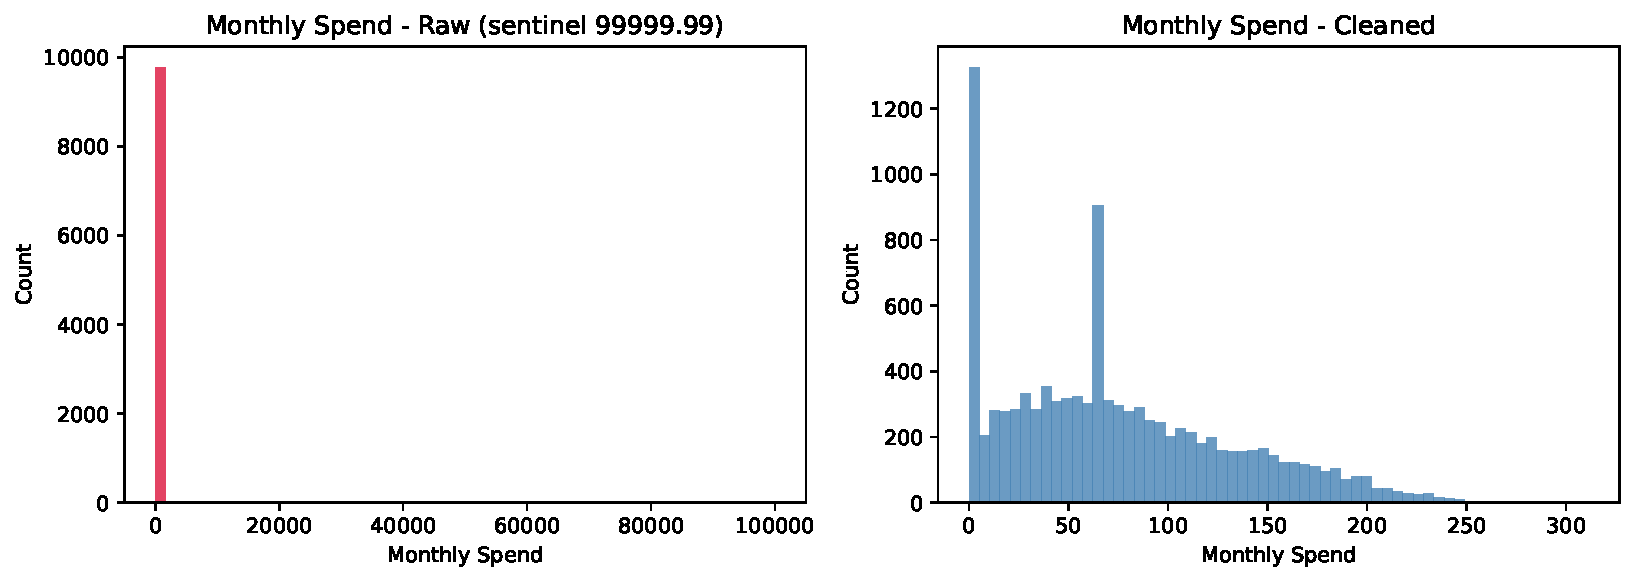
\includegraphics[width=0.95\textwidth]{fig1_data_quality.pdf}
\caption{Effect of cleaning on the \texttt{Monthly\_Spend} distribution. The raw histogram is compressed against the left axis because of the $99{,}999.99$ sentinel; the cleaned histogram reveals the true shape of the variable.}
\label{fig:quality}
\end{figure}

\section{Methodology}
Our analysis combines hypothesis testing, descriptive visualization, and supervised modeling:

\begin{enumerate}
    \item \textbf{Hypothesis tests.} For each numeric feature we use Welch's two-sample $t$-test to compare churners vs.\ retainers. For each categorical feature we use a $\chi^2$ test of independence on the (category $\times$ churn) contingency table.
    \item \textbf{Behavioral signature.} We bin \texttt{Days\_Since\_Last\_Login} into seven ranges and \texttt{Customer\_Service\_Calls} into five ranges, and compute the churn rate in each cell.
    \item \textbf{Predictive models.} We encode categorical features with one-hot (drop-first) and train two models on a stratified 75/25 train-test split: (i) a class-balanced Random Forest with 300 trees; (ii) a class-balanced Logistic Regression on standardized features. We report test-set AUC and feature importance.
\end{enumerate}

\section{Results}

\subsection{Categorical predictors}
Table~\ref{tab:chi2} summarizes the $\chi^2$ tests. \texttt{Subscription\_Plan} and \texttt{Region} are strongly associated with churn; \texttt{Gender} and \texttt{Payment\_Method} are not.

\begin{table}[H]
\centering
\caption{$\chi^2$ tests of independence between categorical features and churn.}
\label{tab:chi2}
\begin{tabular}{lrrr}
\toprule
Feature & $\chi^2$ & dof & $p$-value \\
\midrule
Gender            &   1.39 & 3 & $0.708$ \\
Region            &  41.50 & 3 & $5.1 \times 10^{-9}$ \\
Subscription\_Plan & 152.85 & 2 & $6.4 \times 10^{-34}$ \\
Payment\_Method    &   7.15 & 4 & $0.128$ \\
\bottomrule
\end{tabular}
\end{table}

Figure~\ref{fig:cat} displays churn rates by category, with the overall churn rate marked as a dashed reference.

\begin{figure}[H]
\centering
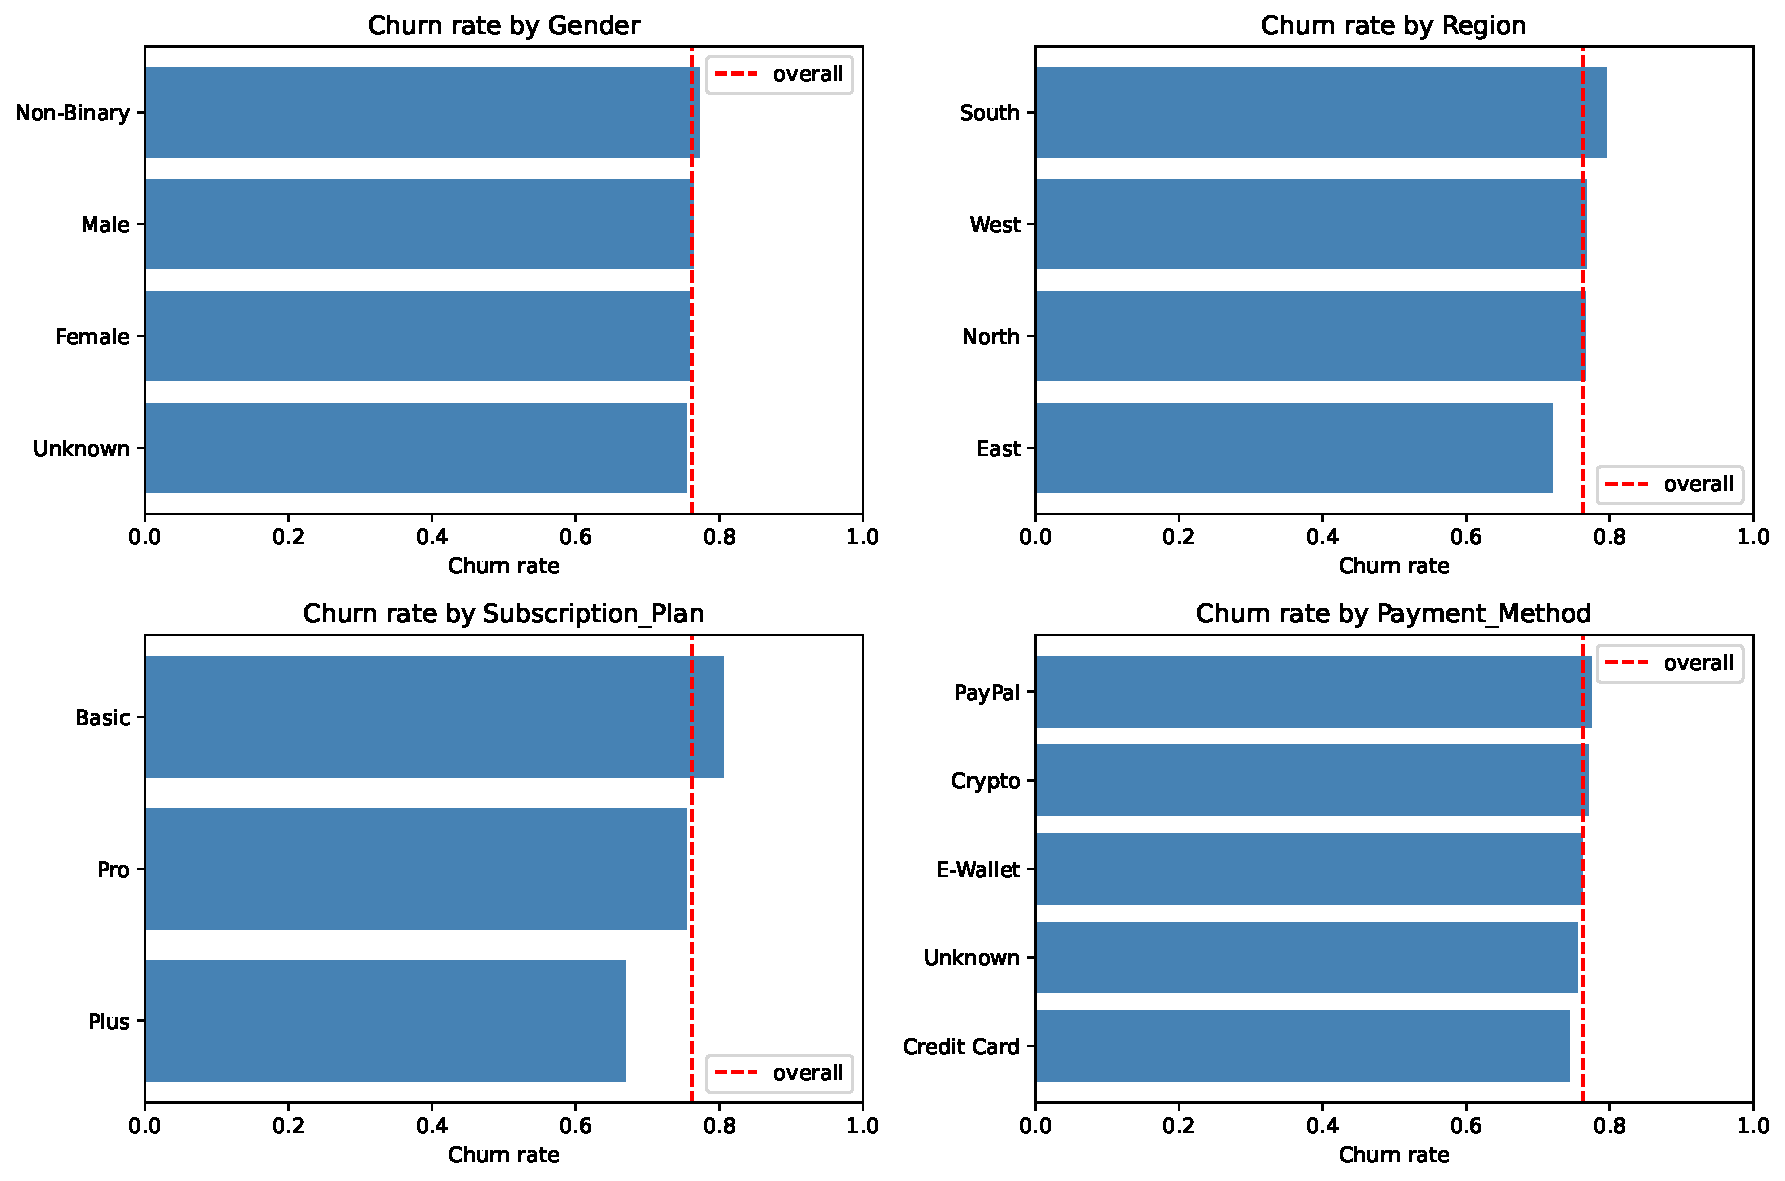
\includegraphics[width=0.95\textwidth]{fig2_churn_by_category.pdf}
\caption{Churn rate by categorical attribute. The red dashed line marks the overall churn rate of $0.762$. \texttt{Subscription\_Plan} shows the largest spread across levels.}
\label{fig:cat}
\end{figure}

\subsection{Numeric predictors}
Table~\ref{tab:ttest} reports Welch's $t$-tests. Three of the four numeric features separate churners from retainers at extreme significance levels; age does not.

\begin{table}[H]
\centering
\caption{Welch's $t$-tests comparing churners vs.\ retainers on numeric features.}
\label{tab:ttest}
\begin{tabular}{lrrrr}
\toprule
Feature & Mean (churn) & Mean (retain) & $t$ & $p$-value \\
\midrule
Age                    &  33.34 &  33.29 &   0.25 & $0.800$ \\
Days\_Since\_Last\_Login &  97.08 &  65.02 &  28.73 & $1.6 \times 10^{-166}$ \\
Customer\_Service\_Calls &   1.91 &   1.39 &  18.57 & $2.3 \times 10^{-74}$ \\
Monthly\_Spend          &  70.60 &  90.55 & $-14.35$ & $1.6 \times 10^{-45}$ \\
\bottomrule
\end{tabular}
\end{table}

\begin{figure}[H]
\centering
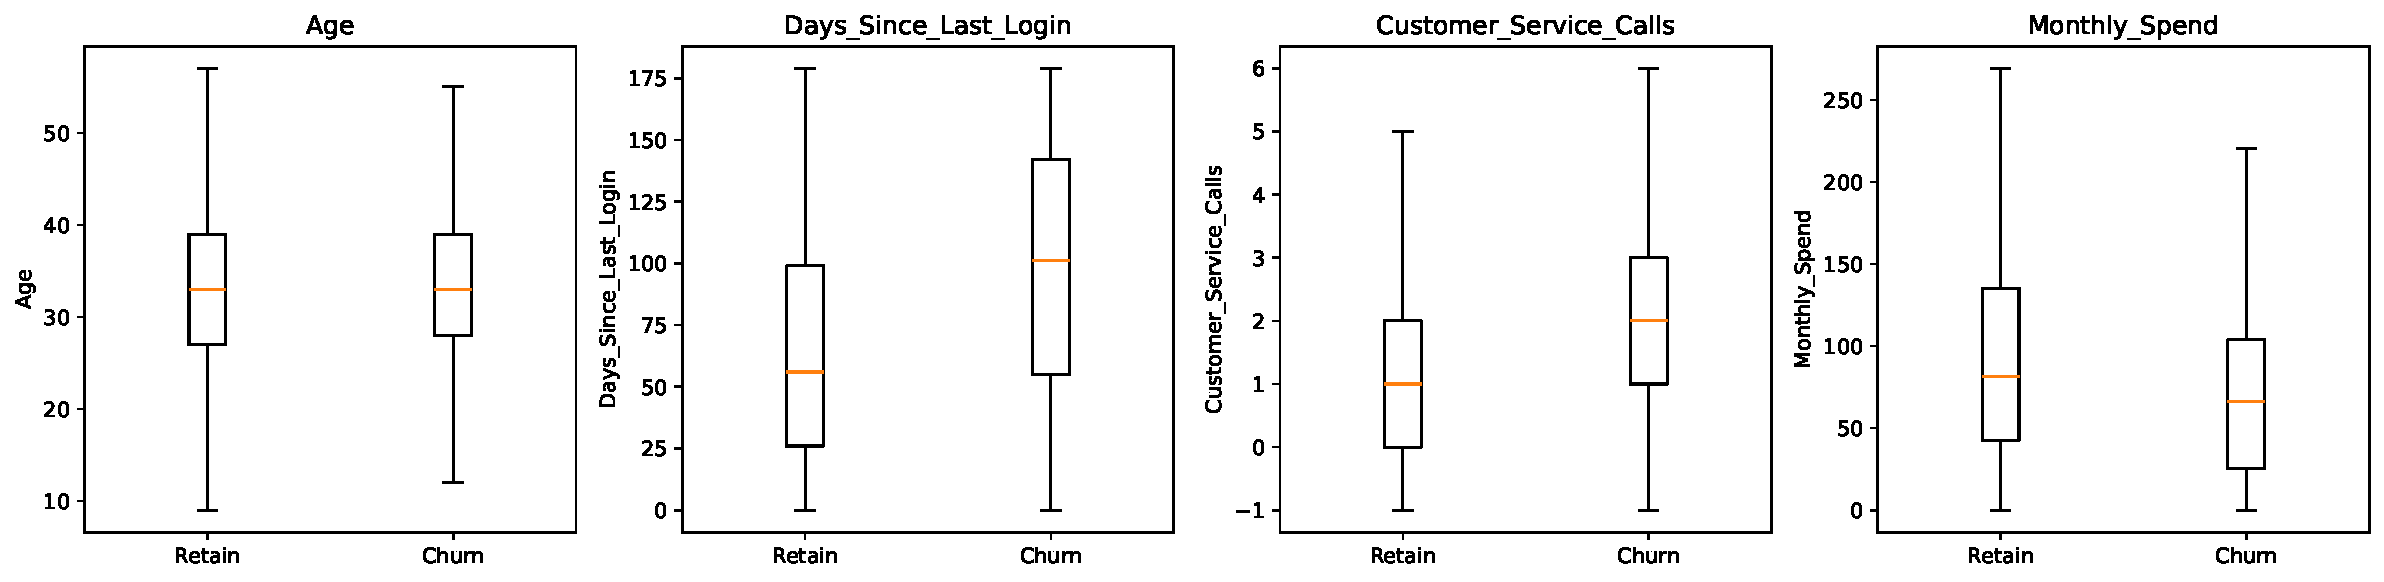
\includegraphics[width=0.95\textwidth]{fig3_numeric_by_churn.pdf}
\caption{Distributions of the four numeric features by churn status. Churners show a higher median days-since-last-login and call count, and a lower monthly spend; age distributions are visually indistinguishable.}
\label{fig:numeric}
\end{figure}

\subsection{Behavioral signature}
Figure~\ref{fig:heatmap} shows churn rates across the joint distribution of \texttt{Days\_Since\_Last\_Login} and \texttt{Customer\_Service\_Calls}. The upper-right region --- customers with long login gaps \emph{and} frequent service calls --- exhibits near-universal churn, whereas the lower-left region --- recently active customers with zero calls --- churns at roughly half that rate. The two axes together define a useful operational early-warning surface.

\begin{figure}[H]
\centering
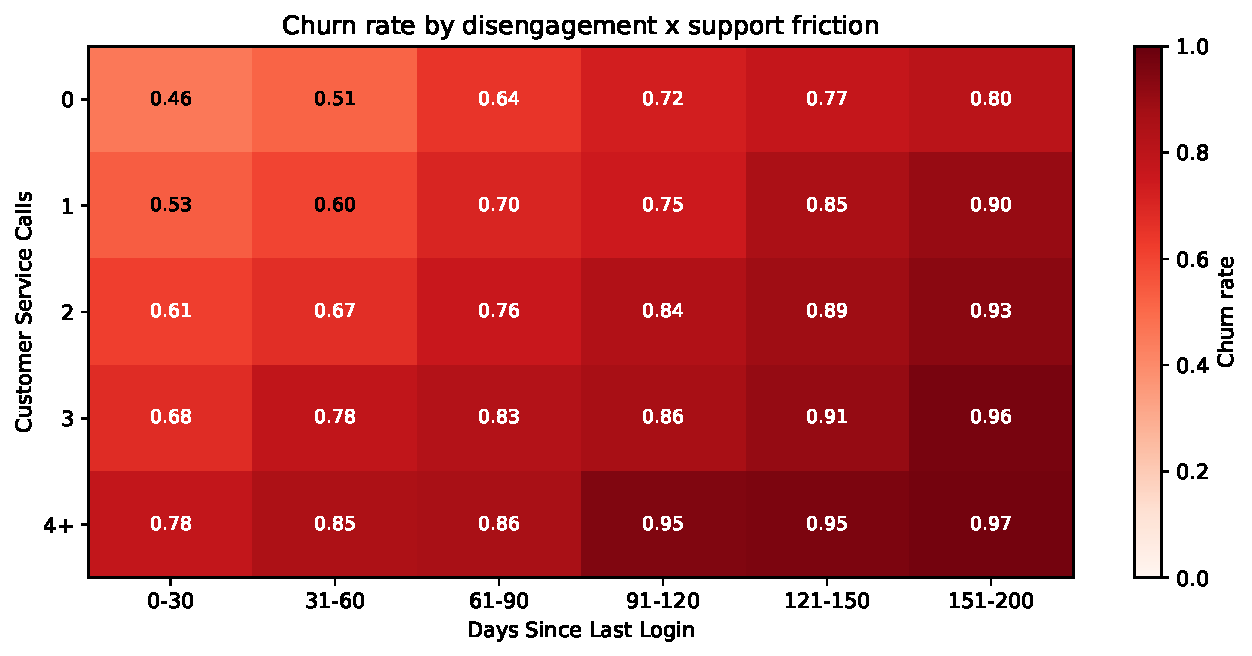
\includegraphics[width=0.85\textwidth]{fig4_behavior_heatmap.pdf}
\caption{Churn rate by disengagement (x-axis) and support friction (y-axis). Darker cells indicate higher churn. The gradient runs from lower-left to upper-right.}
\label{fig:heatmap}
\end{figure}

\subsection{Predictive models}
Both models achieve similar discrimination on the held-out test set: Random Forest AUC $= 0.715$, Logistic Regression AUC $= 0.720$. Figure~\ref{fig:importance} ranks the top 10 Random Forest features; Figure~\ref{fig:roc} shows the ROC curves.

\begin{figure}[H]
\centering
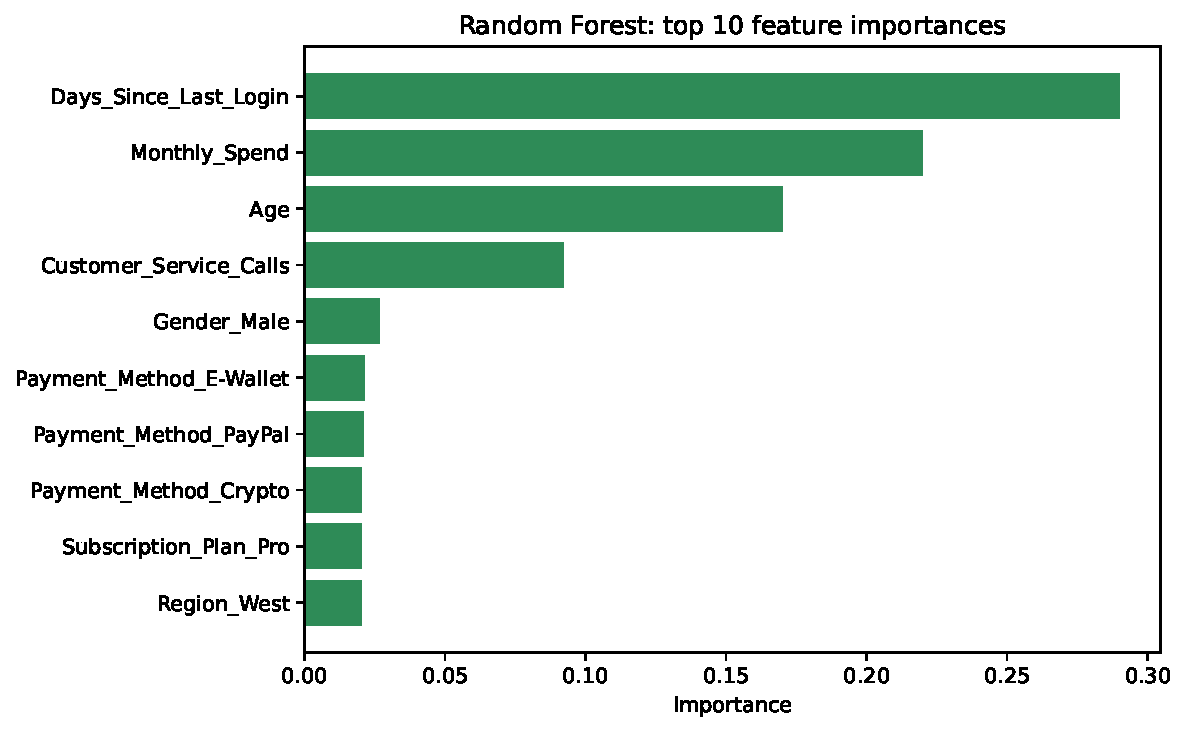
\includegraphics[width=0.8\textwidth]{fig5_feature_importance.pdf}
\caption{Random Forest feature importances. \texttt{Days\_Since\_Last\_Login}, \texttt{Monthly\_Spend}, and \texttt{Age} dominate; one-hot encoded categorical features contribute little individually.}
\label{fig:importance}
\end{figure}

\begin{figure}[H]
\centering
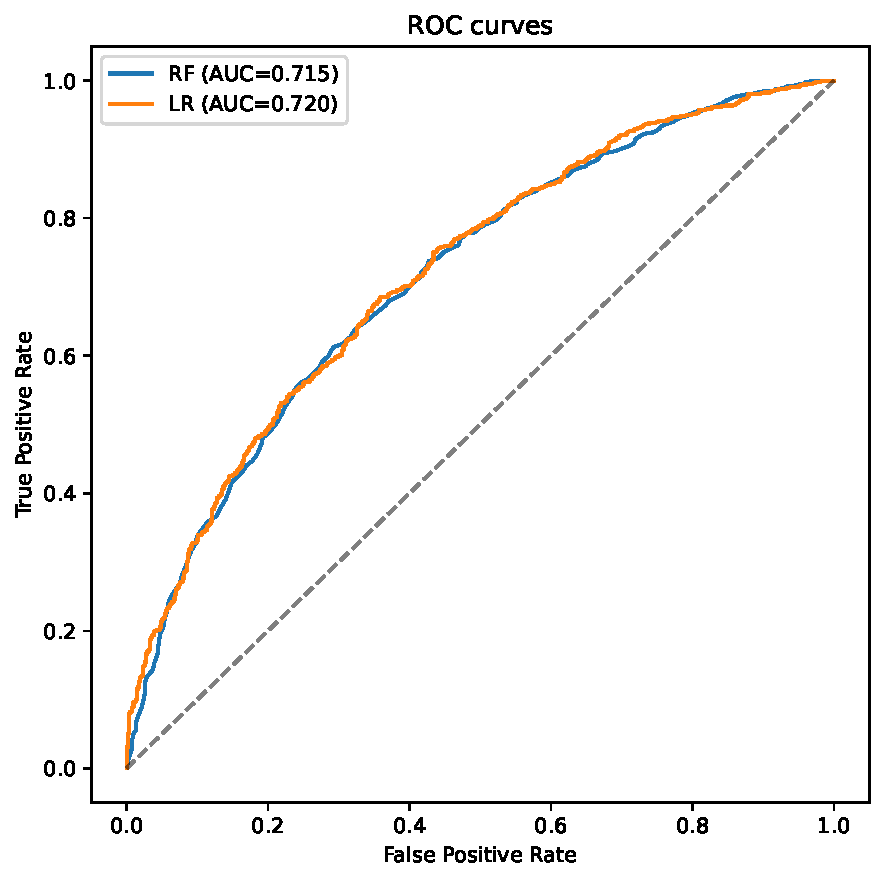
\includegraphics[width=0.6\textwidth]{fig6_roc.pdf}
\caption{ROC curves for Random Forest and Logistic Regression on the 25\% test split. Both achieve AUC $\approx 0.72$.}
\label{fig:roc}
\end{figure}

Logistic regression coefficients (on standardized features) reinforce the interpretation: the largest positive coefficients are \texttt{Days\_Since\_Last\_Login} ($+0.75$) and \texttt{Customer\_Service\_Calls} ($+0.50$); the largest negative coefficient is \texttt{Monthly\_Spend} ($-0.40$). Higher-paying, more recently active customers with fewer support contacts are substantially less likely to churn.

\section{Discussion}
Three findings are noteworthy.

\paragraph{Engagement, not demographics, predicts churn.} Age and gender are statistically uninformative. This suggests that demographic micro-segmentation is a poor retention lever in this dataset; behavioral signals are an order of magnitude stronger.

\paragraph{The behavioral signature is coherent across methods.} The two top features in the $t$-tests (Table~\ref{tab:ttest}), the dominant feature in the Random Forest (Figure~\ref{fig:importance}), and the two largest logistic regression coefficients are the same two variables: \texttt{Days\_Since\_Last\_Login} and \texttt{Customer\_Service\_Calls}. The heatmap in Figure~\ref{fig:heatmap} shows their joint effect directly. This convergence across methods strengthens confidence that the signal is real rather than a modeling artifact.

\paragraph{Data cleaning was outcome-determining.} Without normalization, the case-inconsistent categories would have split statistical power across spurious levels (\texttt{South} vs.\ \texttt{south}). Without sentinel removal, \texttt{Monthly\_Spend} would have had a mean of \$300 and standard deviation of \$4{,}733 (vs.\ \$75 and \$58 after cleaning), which would distort any model that assumes finite variance.

\paragraph{Limitations.} (i) The dataset is cross-sectional: we cannot observe churn timing or ordering of events. (ii) The 76\% churn rate is extreme and may reflect either a truly failing product or a selection-biased sample of at-risk customers; generalization requires knowing which. (iii) Median imputation for 10\% of \texttt{Age} values and 5\% of \texttt{Monthly\_Spend} values attenuates variance; multiple imputation would be preferable. (iv) An AUC of $0.72$ leaves substantial residual variance unexplained, indicating unobserved drivers (product quality, pricing changes, competitor actions).

\section{Conclusion}
In this dataset, customer churn is best predicted by \emph{disengagement} (days since last login), \emph{support friction} (number of customer-service calls), and \emph{lower monthly spend}, in that order. Demographic attributes contribute essentially nothing. A minimal behavioral scorecard built on two variables already stratifies customers into churn-rate bands ranging from roughly 50\% to nearly 100\%, and formal models add only modest incremental lift (AUC $\approx 0.72$). Any production use of this data requires the cleaning protocol described here; naive analysis of the raw file would have produced biased and misleading results.

\end{document}
